\documentclass[letterpaper]{article} % DO NOT CHANGE THIS
\usepackage{aaai2027}  % DO NOT CHANGE THIS
% The serif, sans-serif, and monospaced fonts are loaded automatically by
% aaai2027.sty (newtxtext, helvet, courier). DO NOT add \usepackage{times},
% \usepackage{helvet}, \usepackage{courier}, or any other font package.
\usepackage[hyphens]{url}  % DO NOT CHANGE THIS
\usepackage{graphicx} % DO NOT CHANGE THIS
\urlstyle{rm} % DO NOT CHANGE THIS
\def\UrlFont{\rm}  % DO NOT CHANGE THIS
\usepackage{natbib}  % DO NOT CHANGE THIS AND DO NOT ADD ANY OPTIONS TO IT
\usepackage{caption} % DO NOT CHANGE THIS AND DO NOT ADD ANY OPTIONS TO IT
\frenchspacing  % DO NOT CHANGE THIS
%
% These are recommended to typeset algorithms but not required. See the subsubsection on algorithms. Remove them if you don't have algorithms in your paper.
\usepackage{algorithm}
\usepackage{algorithmic}

%
% These are recommended to typeset listings but not required. See the subsubsection on listing. Remove this block if you don't have listings in your paper.
\usepackage{newfloat}
\usepackage{listings}
\DeclareCaptionStyle{ruled}{labelfont=normalfont,labelsep=colon,strut=off} % DO NOT CHANGE THIS
\lstset{%
	basicstyle={\footnotesize\ttfamily},% footnotesize acceptable for monospace
	numbers=left,numberstyle=\footnotesize,xleftmargin=2em,% show line numbers, remove this entire line if you don't want the numbers.
	aboveskip=0pt,belowskip=0pt,%
	showstringspaces=false,tabsize=2,breaklines=true}
\floatstyle{ruled}
\newfloat{listing}{tb}{lst}{}
\floatname{listing}{Listing}

%
% Recommended for better-looking tables
\usepackage{booktabs}

%
% Keep the \pdfinfo as shown here. There's no need
% for you to add the /Title and /Author tags.
\pdfinfo{
/TemplateVersion (2027.2)
}

% DISALLOWED PACKAGES
% \usepackage{authblk} -- This package is specifically forbidden
% \usepackage{balance} -- This package is specifically forbidden
% \usepackage{CJK} -- This package is specifically forbidden
% \usepackage{float} -- This package is specifically forbidden
% \usepackage{flushend} -- This package is specifically forbidden
% \usepackage{fullpage} -- This package is specifically forbidden
% \usepackage{geometry} -- This package is specifically forbidden
% \usepackage{hyperref} -- This package is specifically forbidden
% \usepackage{navigator} -- This package is specifically forbidden
% (or any other package that embeds links such as navigator or hyperref)
% \usepackage{indentfirst} -- This package is specifically forbidden
% \usepackage{layout} -- This package is specifically forbidden
% \usepackage{multicol} -- This package is specifically forbidden
% \usepackage{nameref} -- This package is specifically forbidden
% \usepackage{savetrees} -- This package is specifically forbidden
% \usepackage{setspace} -- This package is specifically forbidden
% \usepackage{stfloats} -- This package is specifically forbidden
% \usepackage{tabu} -- This package is specifically forbidden
% \usepackage{titlesec} -- This package is specifically forbidden
% \usepackage{tocbibind} -- This package is specifically forbidden
% \usepackage{ulem} -- This package is specifically forbidden
% \usepackage{wrapfig} -- This package is specifically forbidden
% DISALLOWED COMMANDS
% \nocopyright -- Your paper will not be published if you use this command
% \addtolength -- This command may not be used
% \balance -- This command may not be used
% \baselinestretch -- Your paper will not be published if you use this command
% \clearpage -- No page breaks of any kind may be used for the final version of your paper
% \columnsep -- This command may not be used
% \newpage -- No page breaks of any kind may be used for the final version of your paper
% \pagebreak -- No page breaks of any kind may be used for the final version of your paper
% \pagestyle -- This command may not be used
% \tiny -- This is not an acceptable font size.
% \vspace{- -- No negative value may be used in proximity of a caption, figure, table, section, subsection, subsubsection, or reference
% \vskip{- -- No negative value may be used to alter spacing above or below a caption, figure, table, section, subsection, subsubsection, or reference

\setcounter{secnumdepth}{0} %May be changed to 1 or 2 if section numbers are desired.

% The file aaai2027.sty is the style file for AAAI Press
% proceedings, working notes, and technical reports.
%

% Title

\title{Can a Self-Supervised Bird Foundation Model Transfer to Passive-Acoustic Soundscapes? A Diagnostic Study of Bird-MAE on BirdCLEF+ 2025}
\author{
    Author One\textsuperscript{\rm 1},
    Author Two\textsuperscript{\rm 1},
    Author Three\textsuperscript{\rm 1},
    Author Four\textsuperscript{\rm 1}
}
\affiliations{
    \textsuperscript{\rm 1}Nanyang Technological University, Singapore
}


\begin{document}

\maketitle

\begin{abstract}
Self-supervised audio models promise reusable features for passive acoustic monitoring, but it is unclear whether they transfer from clean focal recordings to field soundscapes. We report a diagnostic study of frozen Bird-MAE-Base, a masked-autoencoder transformer pretrained on bird recordings, on the BirdCLEF+ 2025 multi-taxa sound identification task. Every experiment is a change to our team's EfficientNet-B0 baseline (public 0.763, private 0.789) in which only the pretrained model differs. A linear probe on mean-pooled Bird-MAE features reached 0.7495 first-5-second validation AUC (0.7498 on a retry), which would have suggested poor features. The cause was output-bias initialisation: initialising the bias to the class log-prior raised the same linear probe to 0.9626, and the first-epoch loss fell from 0.6941 to 0.0285. A small MLP head reached 0.9749 on validation. Submitted once as a late submission, that head scored 0.77640 public and 0.78016 private, which is 0.013 above the baseline on the public split and 0.009 below it on the private split, so we do not read it as an improvement. Two other pretrained models under the same protocol scored 0.82822/0.81642 (bird-pretrained EfficientNetV2-S) and 0.84774/0.85226 (frozen Perch 2.0 plus an MLP). The gap between clean validation AUC and public leaderboard AUC was 0.1985 for Bird-MAE against 0.1439 for Perch and 0.1550 for the CNN. We discuss three untested hypotheses and the experiments that would test them. Results are from a single seed, and Perch 2.0 was released after the competition closed.
\end{abstract}

\section{Introduction}
Passive acoustic monitoring produces far more audio than experts can annotate. Species identification from such recordings is therefore a natural application for foundation models: networks pretrained once on large audio collections and then reused for many downstream tasks with little labelled data. Self-supervised learning is especially attractive in bioacoustics, because unlabelled or weakly labelled recordings are plentiful, while species labels, and above all labels for continuous soundscapes, are expensive. Masked autoencoders hide most of the input and train a network to reconstruct it \citep{he2021masked}; their audio variants learn from spectrograms without labels \citep{huang2022masked}, and Bird-MAE adapts the idea to bird sound \citep{rauch2025can}. The practical promise is that a frozen encoder plus a light head could replace expensive end-to-end training.

The BirdCLEF+ 2025 competition tests this promise under hard conditions. Participants identify 206 species of birds, amphibians, mammals and insects in every five-second window of one-minute soundscapes from the Middle Magdalena region of Colombia \citep{canas2025birdclef}. The training data are mostly short focal recordings of single species, while the test data are continuous field recordings with overlapping calls, wind, rain and distant sources. A feature extractor that separates species well on clean clips may not do so under these conditions.

Our research question is whether frozen Bird-MAE-Base features, pretrained without species labels on bird recordings, transfer to these soundscapes when a small head is trained on focal clips. We treat it as a diagnostic study. We did not tune Bird-MAE to win; we asked what the number means, and what could make a frozen self-supervised encoder look better or worse than it is. The study is part of a team project for a university course (NTU SC4000) that used the competition for late submissions. Our baseline, v2, is an ImageNet-pretrained EfficientNet-B0 built by a teammate; it scored 0.763 public and 0.789 private. We kept its recipe, data split and inference protocol fixed and changed only the pretrained model. Besides Bird-MAE (A3), two other pretrained models were run under the same protocol and serve as reference points: a bird-pretrained EfficientNetV2-S backbone (A1) and frozen Perch 2.0 embeddings with an MLP head (A2).

To our knowledge, and based on a limited search of the CLEF 2025/2026 BirdCLEF working notes, Kaggle write-ups and arXiv, we found no prior report of frozen Bird-MAE-Base features evaluated on BirdCLEF+ 2025 multi-taxa soundscapes. The coverage of that search was limited (see Related Work and Limitations), so we make no stronger claim.

The contributions are modest and empirical.
\begin{itemize}
\item A leaderboard evaluation of frozen Bird-MAE-Base features with an MLP head on BirdCLEF+ 2025, with public and private scores from one submission, set beside two other pretrained models and the baseline under one protocol.
\item A worked diagnosis of a failure mode of linear probes on frozen features: a low-learning-rate linear probe with default bias initialisation scored 0.7498, and a log-prior bias on the same features gave 0.9626. A first-epoch loss near $\ln 2$ was the early warning.
\item A transfer-gap analysis that compares clean validation AUC with leaderboard AUC for three models, with its limits stated.
\item Three explicitly untested hypotheses for the remaining gap, each paired with the experiment that would test it and with what weakens it.
\end{itemize}

\section{Related Work}
\paragraph{Masked autoencoders for audio.}
Masked autoencoders hide a large fraction of input patches and train a transformer to reconstruct them \citep{he2021masked}. Audio-MAE applied the approach to spectrograms \citep{huang2022masked}. Bird-MAE adapts it to bird sound: it pretrains a ViT on Xeno-canto recordings through the BirdSet resources, reports a new state of the art on the multi-label BirdSet benchmark, and reports that prototypical probes, which use the full patch map, outperform linear probes by up to 37 percentage points of mean average precision on its datasets \citep{rauch2025can}. That figure is for a different metric and different datasets than ours.

\paragraph{BirdSet.}
BirdSet is a large-scale collection for audio classification in avian bioacoustics, with a benchmark of focal-trained models evaluated on soundscape test sets \citep{rauch2025birdset}. It is the benchmark on which Bird-MAE was designed and evaluated. As far as we could see, its evaluation sets are bird soundscapes and do not include the multi-taxa label set of BirdCLEF+ 2025.

\paragraph{Bioacoustic foundation models.}
BirdNET is a deep learning solution for avian diversity monitoring \citep{kahl2021birdnet}. \citet{ghani2023global} showed that global birdsong embeddings enable superior transfer learning for bioacoustic classification. Perch 2.0 continues this line and produces a 1536-dimensional embedding \citep{vanmerrienboer2025perch}; it is described as trained with supervision on recordings from Xeno-canto and iNaturalist. A comparative review covers foundation models for bioacoustics \citep{schwinger2025foundation}. Perch 2.0 appeared after the BirdCLEF 2025 competition closed.

\paragraph{BirdCLEF and winning approaches.}
BirdCLEF is the bird and wildlife identification task of the LifeCLEF campaign. The 2025 edition is scored by macro-averaged ROC-AUC \citep{canas2025birdclef}. The second-place team combined a strong baseline, in-domain transfer learning, semi-supervised distillation against domain shift, postprocessing and ensembling, and reported ROC-AUC of 0.928 private and 0.925 public \citep{sydorskyi2025tackling}. We use their released pretrained backbone in A1 and nothing else from their system. Another team distilled spectrograms into tokens for a fast, lightweight classifier \citep{miyaguchi2025distilling}. BirdCLEF+ 2026 working notes continue to stress runtime and domain shift \citep{banthia2026pantanal,chen2026class}. We read these papers for context and use none of their numbers for comparison.

\paragraph{Prior use of Bird-MAE on BirdCLEF.}
We searched for earlier evaluations of Bird-MAE on BirdCLEF data. The search covered the titles and abstracts of the four BirdCLEF+ papers in the 2025 CEUR volume, the index of the 2026 working notes, one 2026 paper that mentions Bird-MAE in its discussion but does not evaluate it, Kaggle search for write-ups, and arXiv. We found no report of frozen Bird-MAE-Base on BirdCLEF+ 2025. The search was limited: the full text of the four 2025 papers and of most 2026 papers could not be read with our tools, and Kaggle notebooks and discussion threads were not searchable. Absence of a hit is therefore weak evidence.

\paragraph{Transfer learning and backbones.}
EfficientNet and EfficientNetV2 trade accuracy against size and speed \citep{tan2019efficientnet,tan2021efficientnetv2}. v2 uses the B0 member with ImageNet weights and A1 the V2-S member. Mixup is part of v2's augmentation \citep{zhang2018mixup}. Time-frequency masking in the style of SpecAugment is a common audio augmentation \citep{park2019specaugment} that v2 does not use. Distillation and noisy-student training \citep{hinton2015distilling,xie2020selftraining} are relevant to future work only.

\section{Task and Data}
The competition provides a labelled set of short focal recordings (\texttt{train\_audio}), unlabelled soundscapes (\texttt{train\_soundscapes}) and a hidden test set of about 700 one-minute soundscapes. The label space has 206 classes: 146 birds, 34 amphibians, 17 insects and 9 mammals. For each test soundscape the system outputs 12 rows, one per five-second window, with a probability for every class. The metric is macro-averaged ROC-AUC over classes, skipping classes with no positive example in the evaluated set. Kaggle scores a submission on two disjoint parts of the hidden test set, called public and private. A late submission is scored like an on-time one but does not count for ranking. The submission notebook must run on CPU in at most 90 minutes with internet off; we set an internal budget of 75 minutes.

Our validation uses a stratified 80/20 split of the focal clips with seed 42, giving 22,851 training and 5,713 validation clips; 191 of the 206 classes have at least one positive in the validation set. We report two protocols. ``First-5s'' scores the first five seconds of each validation clip against its primary label. ``Clip-max'' takes the class-wise maximum over all windows of a clip of up to 30 s. The first-5s protocol was inherited from the baseline, and every headline validation number below uses it. No labelled soundscapes are available, so no local validation reflects the test conditions directly.

\section{Methods}
\subsection{Bird-MAE pipeline}
\paragraph{Encoder.}
Bird-MAE-Base is a ViT-B/16 with 12 transformer layers, 768-dimensional tokens and 85.5M parameters, pretrained as a masked autoencoder \citep{rauch2025can}. We used the public checkpoint \texttt{DBD-research-group/Bird-MAE-Base} at a fixed commit, with every file verified by SHA-256 and the model loaded from a local copy with a pinned version (4.38.0) of the transformers library. The encoder was frozen and never trained.

\paragraph{Input.}
The model's own feature extractor computes a Kaldi-style filterbank with 128 mel bins and a 10 ms frame shift, and pads or truncates to 512 frames, which corresponds to a five-second window at 32 kHz. The input tensor is $1\times512\times128$ after normalisation with fixed constants, which gives $32\times8=256$ patches of size $16\times16$. Because BirdCLEF windows match the native five-second length, we cut raw audio at 32 kHz without resampling. This front end differs from the log-mel front end of our baseline, so the baseline's cached spectrograms could not be reused and features were computed from audio. The repository pads short inputs with the minimum value of whatever batch is passed in. To keep a window's input independent of its neighbours, and identical in training and inference, we called the feature extractor once per window and never on a batch.

\paragraph{Embedding.}
The encoder returns the mean of its patch tokens followed by a layer normalisation, a 768-dimensional vector per window; no class token was used. For each focal clip we embedded up to the first 30 s as non-overlapping five-second windows, giving 106,157 windows from 28,564 clips, with automatic mixed precision on a T4 GPU. Embeddings were cached to disk once and all heads were trained from the cache.

\paragraph{Heads.}
Features were standardised with the training-row mean and standard deviation. The linear head maps 768 dimensions to 206 logits. The MLP head has one hidden layer of 512 units with ReLU and dropout 0.2. Both were trained with binary cross-entropy, targets of 1.0 for the primary label and 0.5 for secondary labels, and a loss in which each window is weighted by the reciprocal of its clip's window count, so that each clip contributes equally. The optimiser was AdamW with weight decay 0.01, batch size 1,024 and a one-cycle schedule, using v2's split. Linear heads ran 30 epochs. Each reported number is the best epoch by first-5s validation AUC, so it is a selected, mildly optimistic value.

\paragraph{Bias initialisation.}
The output layer computes $z_c = w_c^{\top}x + b_c$ for class $c$. Most classes are absent from most windows, so the correct starting prediction for most classes is a small probability. Default initialisation puts the bias near zero (measured mean $-0.0021$ in the MLP run and $0.0009$ in the linear retry), which starts every class at probability 0.5. The alternative sets $b_c=\log\frac{p_c}{1-p_c}$, with $p_c$ the weighted fraction of training windows in which class $c$ is labelled, a standard remedy that \citet{lin2017focal} use in an object detector. A uniform-class estimate would put the bias at $\log(1/206)=-5.3$. The measured mean log-prior on our features is $-6.2008$ (minimum $-9.3435$, maximum $-3.0985$, no class clipped). The log-prior variant overwrites the final bias in place without drawing random numbers, so the default and log-prior runs share initial weights and batches and differ only in the bias.

\paragraph{Inference.}
At inference each soundscape is cut into 12 windows, each is passed through the feature extractor separately, and the 12 are batched through the encoder on CPU with one thread, in four file-level worker processes, followed by the head in numpy. Sigmoid outputs are written with no post-processing.

\subsection{Reference systems}
\paragraph{Baseline v2.}
v2 is an EfficientNet-B0 with ImageNet weights on a log-mel input (128 bands, $n_\mathrm{fft}=2048$, hop 512, 50--14,000 Hz at 32 kHz, decibels relative to the window maximum over an 80 dB range, scaled to $[0,1]$). Training took random five-second crops of cached spectrograms, added noise from unlabelled soundscapes with probability 0.5 at $-20$ to $-3$ dB, and used mixup with probability 0.5 \citep{zhang2018mixup}. The loss was binary cross-entropy with AdamW at $10^{-3}$ under a one-cycle schedule, batch size 64 and 15 epochs. Its validation AUC was not recorded in the notebooks we hold.

\paragraph{A1.}
A1 replaces the B0 with the 2025 \texttt{tf\_efficientnetv2\_s\_in21k} backbone pretrained on bird audio by the second-place team \citep{sydorskyi2025tackling}, fine-tuned end to end with v2's recipe. It is a backbone change and not a weights-only swap. The pretrained weights loaded for 774 of 780 keys; the missing keys reported in the log belong to the \texttt{conv\_head} and \texttt{bn2} layers, which were trained from random initialisation. Its normalisation only partly matches the pretraining front end.

\paragraph{A2.}
A2 freezes Perch 2.0 \citep{vanmerrienboer2025perch}, used through a community ONNX conversion pinned to a commit and a hash. It embeds a five-second window as a 1536-dimensional vector, on which we trained an MLP head (512 hidden units, dropout 0.3, 30 epochs, learning rate $10^{-3}$, same targets, weighting and split) over the same 106,157 windows. Perch's own class logits were not used. The head was trained on embeddings of clean focal clips without any augmentation; its only regularisation was dropout. We checked this in the embedding notebook, which contains no noise, mixing or masking step.

\section{Experimental Setup}
Feature extraction and end-to-end training ran on Kaggle T4 GPUs. The Bird-MAE embedding notebook used about 0.3 GPU hours by our record (an estimate; the log shows a session wall time of 0.24 h). Head training and sweeps ran on Kaggle CPU from the cached features. Every experiment used one seed and one split. A3 was submitted to Kaggle once, and public and private scores are reported together. Differences below 0.01 on the public leaderboard are treated as noise. Before submitting, a 20-file dry run on unlabelled soundscapes projected the 700-file CPU runtime, and a submission was allowed only if the projection was at most 75 minutes. Kaggle's command-line interface does not report the scored runtime, so every CPU time for a submitted notebook in this paper is a projection, not a scored-run measurement.

The Bird-MAE head was selected by clean validation AUC alone, because only one A3 submission was made. In particular, the choice between the default-bias and log-prior MLPs was made on validation and not on the leaderboard.

\section{Results}
The results follow the order in which the diagnosis unfolded. Figure~\ref{fig:arc} summarises the validation AUC at each stage.

\begin{figure}[t]
\centering
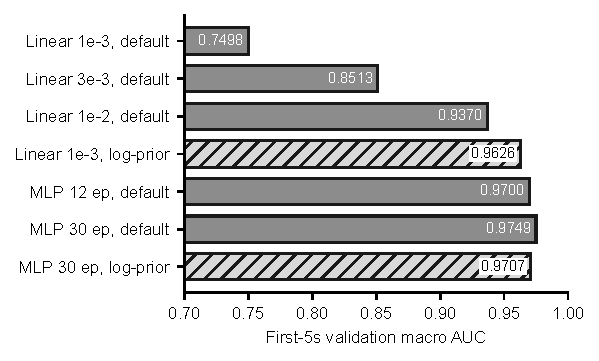
\includegraphics[width=\columnwidth]{figures/diagnostic_arc.pdf}
\caption{First-5s validation AUC of heads on frozen Bird-MAE-Base features. Plain bars use the default bias, hatched bars the log-prior bias. Learning rates are maximum one-cycle rates. Linear rows ran 30 epochs and the 12-epoch MLP row 12; the epoch counts are not matched. The horizontal axis starts at 0.70.}
\label{fig:arc}
\end{figure}

\subsection{A linear probe that looked poor}
The first probe was a linear head on standardised mean-pooled features, with learning rate $10^{-3}$ and 30 epochs. It reached 0.7495 first-5s validation AUC (clip-max 0.716). A later rerun on the cached features reproduced the figure within 0.0003: 0.7498 first-5s and 0.7183 clip-max. The standard reading of such a result, and the one the Bird-MAE paper invites, is that pooled features are a weak interface for the model \citep{rauch2025can}.

The training loss gave a different picture. It began at 0.6929 in the first run (0.6941 in the retry), close to $\ln 2=0.693$, the loss of predicting probability 0.5 for every class, and it fell slowly to a plateau of 0.2770 after 30 epochs. A loss near $\ln 2$ at the start is expected for default initialisation. A plateau at 0.277 is not a statement about the features: a head that had merely learned the class base rates would reach a far lower loss, as the log-prior run below shows (0.0285 in its first epoch). The plateau therefore indicates that the output offset had not been learned.

\subsection{Learning-rate sweep}
We ran a sweep of heads on the cached features (Table~\ref{tab:sweep}). Raising the linear learning rate from $10^{-3}$ to $3\times10^{-3}$ and $10^{-2}$ raised first-5s AUC from 0.7498 to 0.8513 and 0.9370, and removing standardisation at $10^{-3}$ gave 0.8158. The best entries were MLP heads: 0.9700 at learning rate $3\times10^{-3}$ and dropout 0.2, and 0.9697 at dropout 0.5. The MLP rows ran 12 epochs and the linear rows 30, so the comparison is not epoch-matched, and the sweep did not save a head. That a larger step size removed most of the gap hinted that the optimiser, and not the features, limited the linear probe.

\begin{table}[t]
\centering
\small
\begin{tabular}{llcc}
\toprule
Head & Settings & First-5s & Clip-max \\
\midrule
MLP & $3\times10^{-3}$, drop 0.2 & 0.9700 & 0.9697 \\
MLP & $3\times10^{-3}$, drop 0.5 & 0.9697 & 0.9693 \\
Linear & $10^{-2}$ & 0.9370 & 0.9183 \\
MLP & $10^{-3}$, drop 0.2 & 0.9305 & 0.9319 \\
MLP & $10^{-3}$, drop 0.5 & 0.9263 & 0.9274 \\
Linear & $3\times10^{-3}$ & 0.8513 & 0.8250 \\
Linear & $10^{-3}$, no standardisation & 0.8158 & 0.8467 \\
Linear & $10^{-3}$, standardised & 0.7498 & 0.7183 \\
\bottomrule
\end{tabular}
\caption{Head sweep on cached Bird-MAE features with default bias. MLP rows ran 12 epochs, linear rows 30. Settings give the maximum learning rate and dropout.}
\label{tab:sweep}
\end{table}

\subsection{Bias initialisation as the cause}
The learning-rate result suggested a bias problem. The default bias starts near 0, while the log-prior of a typical class is $-6.2008$ on these features, and $\log(1/206)=-5.3$ under a uniform-class estimate; we give both because the second is a convenient hand estimate and the first is measured. A code review estimated that, at a maximum learning rate of $10^{-3}$ over about 2,340 steps under the one-cycle schedule, an Adam-style update could move a bias by about 1.3 in total. That figure is an analytical estimate from the review and was not measured from a run. Under it the bias cannot reach $-5$ or $-6$, and a linear head, which has no other free offset, plateaus. The same review predicted a plateau loss of about 0.25 to 0.28, against 0.277 observed.

The test was to change only the bias (Table~\ref{tab:bias}). With the log-prior bias and the same learning rate, the linear probe reached 0.9626 first-5s (clip-max 0.9636), and the first-epoch loss was 0.0285 instead of 0.6941. At a learning rate of $3\times10^{-3}$ the log-prior probe reached 0.9618. The single change took the same features from 0.7498 to 0.9626. This supports bias initialisation as the main cause, but it is one experiment with one seed, and we did not measure the actual bias trajectory.

\begin{table}[t]
\centering
\small
\begin{tabular}{llccc}
\toprule
Head & Bias & First-5s & Clip-max & Ep.~1 loss \\
\midrule
Linear $10^{-3}$ & default & 0.7498 & 0.7183 & 0.6941 \\
Linear $10^{-3}$ & log-prior & 0.9626 & 0.9636 & 0.0285 \\
Linear $3\times10^{-3}$ & log-prior & 0.9618 & 0.9631 & 0.0265 \\
MLP, 30 ep & default & 0.9749 & 0.9748 & 0.2760 \\
MLP, 30 ep & log-prior & 0.9707 & 0.9708 & 0.0262 \\
\bottomrule
\end{tabular}
\caption{Output-bias initialisation on frozen Bird-MAE features (validation only). Linear heads ran 30 epochs.}
\label{tab:bias}
\end{table}

\subsection{MLP heads}
We then trained the MLP head for 30 epochs under the same protocol, twice from the same seed, once with default bias and once with log-prior bias. The default-bias run reached 0.9749 first-5s AUC (best epoch 26, clip-max 0.9748). Its 12-epoch counterpart in the sweep scored 0.9700, so the longer schedule added 0.0049. The log-prior run reached 0.9707 (best epoch 10, clip-max 0.9708), which is 0.0042 lower. The log-prior bias that rescued the linear head did not help the MLP. The default-bias MLP's first-epoch loss was 0.2760 and it fell to 0.0294 in the second epoch, while the log-prior MLP began at 0.0262, consistent with a hidden layer that can supply a large negative offset to every logit. We did not test that explanation, and why the log-prior start was slightly worse than the default one is not recorded. Retraining both heads on CPU took 101 s (default) and 91 s (log-prior). The default-bias MLP won on validation and is the head that was submitted.

\subsection{Leaderboard}
Table~\ref{tab:lb} and Figure~\ref{fig:lb} give the leaderboard scores. The Bird-MAE head scored 0.77640 public, which clears the 0.776 grading cut-off by 0.0004, a margin well inside the noise level, and 0.78016 private, which is 0.009 below v2. The public gain of +0.013 over v2 is only slightly above our 0.01 noise threshold, and the private change has the opposite sign, so we do not read A3 as an improvement over the baseline. The other two models gained +0.065 and +0.085 public, and A1 and A2 cleared the 0.810 team goal on both splits. No ensemble was tested and no official ranking is claimed.

\begin{table}[t]
\centering
\small
\begin{tabular}{lcccc}
\toprule
Model & Val & Public & Private & $\Delta$ pub. \\
\midrule
v2 (B0) & not rec. & 0.763 & 0.789 & 0 \\
A1 V2-S, bird & 0.9832 & 0.82822 & 0.81642 & +0.065 \\
A2 Perch 2.0 & 0.9916 & \textbf{0.84774} & \textbf{0.85226} & +0.085 \\
A3 Bird-MAE & 0.9749 & 0.77640 & 0.78016 & +0.013 \\
\bottomrule
\end{tabular}
\caption{Leaderboard results of one submission each. Val is first-5s validation AUC (A1 at its best epoch). Private differences from v2 are +0.027 (A1), +0.063 (A2) and $-0.009$ (A3). Grading cut-off 0.776 (public), team goal 0.810.}
\label{tab:lb}
\end{table}

\begin{figure}[t]
\centering
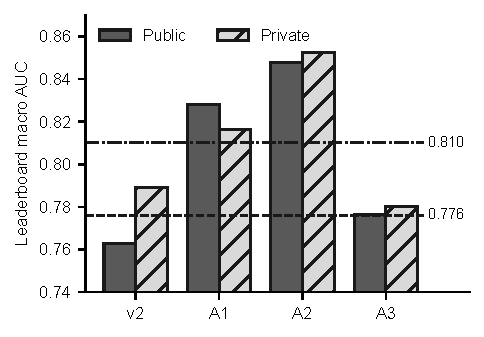
\includegraphics[width=\columnwidth]{figures/leaderboard_compare.pdf}
\caption{Public and private leaderboard scores. The dashed line is the grading cut-off (0.776, public) and the dash-dot line the team goal (0.810). The vertical axis starts at 0.74.}
\label{fig:lb}
\end{figure}

\subsection{Cost}
Embedding the 106,157 windows took 691 s of wall time on a T4 (363 s in the model call, 154 windows per second). The whole GPU session lasted 0.24 h in the log, and we recorded about 0.3 GPU hours as an estimate. Inference on CPU was the slowest of the three models. A 20-file dry run gave 5.25 s per file with four workers, which projects to 61.6 minutes for 700 files. Summed over workers, the 20 files took 100.9 s for the mel front end and 313.6 s for the encoder, with 0.68 s for the head and 17.6 s of model loading per worker. For comparison, A1's submitted notebook projects to about 37 minutes and A2's to 25.0 minutes under the same dry-run method, and the baseline's own notebook was measured at 11.1 minutes for 700 files. All three projections are below the 75-minute budget, but Bird-MAE leaves the least headroom, so even a better head would have left little room for a second model in an ensemble. The A1 projection is likely pessimistic because worker start-up is spread over only 20 files.

\subsection{Transfer gap}
Table~\ref{tab:gap} and Figure~\ref{fig:gap} subtract the leaderboard AUC from the first-5s validation AUC. Bird-MAE's gap, 0.1985 public and 0.1947 private, was the largest of the three models on both splits. A2 had the smallest and A1 was in between. A1 and A2 differ by 0.0111 public and 0.0275 private, a difference we do not interpret.

\begin{table}[t]
\centering
\small
\begin{tabular}{lcccc}
\toprule
Model & Val & Public & Gap pub. & Gap priv. \\
\midrule
v2 & not rec. & 0.763 & n/a & n/a \\
A1 & 0.9832 & 0.82822 & 0.1550 & 0.1668 \\
A2 & 0.9916 & 0.84774 & 0.1439 & 0.1393 \\
A3 & 0.9749 & 0.77640 & 0.1985 & 0.1947 \\
\bottomrule
\end{tabular}
\caption{Validation minus leaderboard AUC, first-5s validation, four decimals. Single seed and single split. Validation is macro AUC over held-out focal clips (191 classes with positives) and the leaderboard is macro AUC on soundscapes over a different class set, so the difference mixes domain shift with class coverage and is descriptive only. A2's validation AUC may be inflated by overlap between Perch's training data and the competition's training audio, which would widen its gap. The v2 row is unavailable because its validation AUC was not recorded.}
\label{tab:gap}
\end{table}

\begin{figure}[t]
\centering
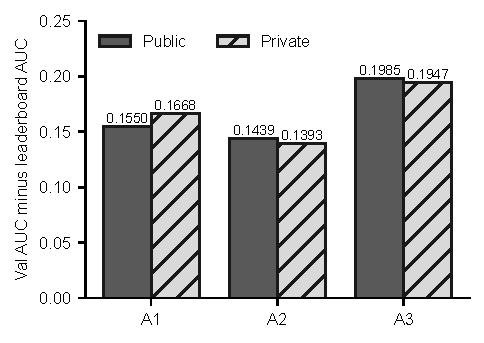
\includegraphics[width=\columnwidth]{figures/transfer_gap.pdf}
\caption{Validation AUC minus leaderboard AUC for the three pretrained models, public and private splits.}
\label{fig:gap}
\end{figure}

\section{Discussion}
\subsection{What the diagnostic shows}
Three things are supported by our data, within the limits of one seed. First, the linear probe at 0.7498 was a result about the optimiser and the output bias and not about the features: the same features gave 0.9626 with a log-prior bias. Second, even with the bias repaired, and with the head that had the best validation AUC (0.9749), the Bird-MAE features gave a small public gain over the baseline (+0.013) and a private loss ($-0.009$). Third, clean validation AUC ordered the three encoders as the leaderboard did but compressed the differences: validation AUCs of 0.9916, 0.9832 and 0.9749 span 0.017, while public scores of 0.84774, 0.82822 and 0.77640 span 0.071. The remaining question is why Bird-MAE transferred worse, and we do not know.

\subsection{Hypotheses (untested)}
The following are hypotheses. None was tested here. Each is given with the experiment that would test it and with what weakens it.

\paragraph{H1: mean pooling dilutes short calls.}
Mean pooling averages 256 patch tokens, and a short call occupies few patches, so the pooled vector may be dominated by background in a noisy soundscape window. The Bird-MAE paper reports that prototypical probes on the full patch map beat linear probes on pooled features by up to 37 percentage points of mean average precision on its benchmark \citep{rauch2025can}. Test: replace mean pooling by attention or max pooling over cached patch tokens, or train a prototypical probe, and compare the transfer gap. What weakens it: the 37-point figure is for a different metric and datasets, and our head is an MLP and not a linear probe. Perch's embedding also aggregates each window into one vector, so pooling alone cannot explain why that representation transferred better. H1 is rather about pooling a patch map after the fact versus using an encoder trained end to end to produce that single output.

\paragraph{H2: the head saw only clean-clip features.}
The head was trained on embeddings of clean focal clips, with no noise augmentation, and then applied to noisy soundscape windows, where features may shift. Our baseline did add soundscape noise during training. Test: embed focal clips after mixing in soundscape noise at the baseline's levels, retrain the head, and measure the gap. What weakens it: A2's head was trained in the same way, on clean-clip embeddings with no augmentation, and it transferred best. H2 alone therefore cannot explain the difference between A2 and A3, although it may interact with the encoder, for example if one encoder's features are more sensitive to added noise than the other's.

\paragraph{H3: pretraining objective and data.}
Bird-MAE was pretrained without labels on a Xeno-canto snapshot, as described in the sources we read, which treat it as bird data; we did not confirm the taxonomic composition \citep{rauch2025can,rauch2025birdset}. Perch 2.0 is described as trained with supervision on Xeno-canto and iNaturalist recordings, and we did not verify its taxonomic composition either \citep{vanmerrienboer2025perch}. A supervised objective may give embeddings that separate species under noise, in line with earlier evidence for supervised bird embeddings \citep{ghani2023global}, and a bird-only pretraining set may serve the non-bird classes less well. Test: the leaderboard does not give per-taxon AUC, so the test needs a labelled soundscape subset, on which per-taxon AUC for birds and non-birds could be compared across encoders, or a supervised bird-only encoder as a control. What weakens it: the two models also differ in size, training data volume and release date, so any difference may be due to one of these and not to the objective. A2's validation AUC may also be inflated by data overlap, as noted above.

\subsection{Interactions between the hypotheses}
The hypotheses are not exclusive. A model whose features are diluted by pooling (H1) and shifted by noise (H2) could be hit harder when the head is also trained only on clean data. We cannot separate them with a single submission per model. We also note that the validation difference between A1 and A3 is 0.0083, while the public difference is 0.0518 (0.82822 against 0.77640), so clean validation understates leaderboard differences for this pair. A1 is confounded, since it changes the architecture, the pretraining and the normalisation together, and is used here as a reference point only.

\subsection{The Perch plateau}
The Perch logistic regression showed the same loss plateau (0.278) as the Bird-MAE linear probe (0.277) and a lower validation AUC than the Perch MLP (0.9071 against 0.9916). Bias initialisation was not re-tested for Perch, so that its linear score has the same defect is presumed and not shown. The MLP was the head submitted for Perch, so this does not affect the leaderboard figure.

\subsection{Practical lessons}
These lessons come from one case, and we offer them as practice and not as findings.
\begin{itemize}
\item Check the first-epoch loss against $\ln 2$. A start near 0.693 on a multi-label problem with rare classes means the model begins at probability 0.5 everywhere, and a plateau well above zero afterwards points at the output offset rather than at the features.
\item Initialise the output bias of rare multi-label classes to the log-prior before judging frozen features with a linear head. This took our probe from 0.7498 to 0.9626. It did not help our MLP (0.9707 against 0.9749), so we treat it as a diagnostic step and not as a default.
\item Keep a domain-matched evaluation. Without labelled soundscapes we could not tell whether a head suited the target domain, and the leaderboard was the only domain-matched check.
\item Do not rank encoders by clean validation AUC. In our table it ordered the models correctly but compressed a 0.071 public spread into a 0.017 validation spread, and with a different set of models the order could differ.
\end{itemize}

\section{Limitations}
\begin{itemize}
\item \textbf{Single seed and no error bars.} Each configuration was trained once and submitted once. We cannot estimate run-to-run variance, so small differences should not be interpreted.
\item \textbf{Untested hypotheses.} H1 to H3 are conjectures. The only causal result here is the bias-initialisation one, and its bias-travel estimate of about 1.3 is analytical.
\item \textbf{Leaderboard noise.} Public differences below 0.01 are treated as noise. A3's margin over the grading cut-off (0.0004) is in that range, and its public gain over v2 (+0.013) is only slightly above it.
\item \textbf{Perch 2.0 and the competition.} Perch 2.0 was released after BirdCLEF 2025 closed, so A2 is not comparable to official ranks of that competition. We make no ranking claim.
\item \textbf{Training-data overlap.} Perch's training data and the competition's training audio may share recordings, which can inflate A2's validation AUC and widen its gap. We did not check the overlap.
\item \textbf{Licence.} The Bird-MAE weights have no declared licence on the model card, the code repository or the arXiv listing. We kept them in a private dataset and did not redistribute them.
\item \textbf{No labelled soundscapes.} Domain-shift explanations could not be tested directly, and the transfer gap mixes domain shift with class coverage.
\item \textbf{Selection on clean validation.} The A3 head was selected by clean validation AUC, with no leaderboard selection and one submission.
\item \textbf{Prototypical probe not run.} The probe that the Bird-MAE paper favours was not tried, so the A3 result describes mean pooling with an MLP head only.
\item \textbf{Limited novelty search.} The full text of most working notes and Kaggle notebooks was not covered (see Related Work).
\item \textbf{Timing and A1.} CPU runtimes of submitted notebooks are projections from 20-file dry runs. A1 confounds architecture, pretraining and normalisation. The baseline's validation AUC was not recorded.
\end{itemize}

\section{Future Work}
The most direct next steps follow the hypotheses: a pooling ablation over cached patch tokens (H1), noise-augmented embedding of the training clips (H2), and a labelled soundscape subset for per-taxon evaluation (H3). A prototypical probe would follow, and fine-tuning Bird-MAE with noise augmentation if the probe is competitive. A log-prior-initialised linear head on Perch would close the open question about the Perch plateau. A noisy-student loop with a teacher built from A1 and A2 is a further direction: the teacher would label the unlabelled soundscapes and a noised student would train on them \citep{xie2020selftraining,hinton2015distilling}. This was not built, and we make no claim about such a teacher.

\section{Conclusion}
Frozen Bird-MAE-Base features with an MLP head scored 0.77640 public and 0.78016 private on BirdCLEF+ 2025 in one late submission, which is slightly above our baseline on the public split, below it on the private split, and well below frozen Perch 2.0 (0.84774 and 0.85226) under the same protocol. A linear probe that scored 0.7498 on validation reached 0.9626 once the output bias was initialised to the class log-prior, so the first number reflected the initialisation and not the features. Even after that repair, the gap between clean validation AUC and leaderboard AUC was largest for Bird-MAE, at 0.1985 on the public split. We offered three untested hypotheses, on pooling, clean-only head training and pretraining objective, each with a test. The evidence rests on one seed, one split and one submission per model, and Perch 2.0 post-dates the competition, so these results are a diagnostic record and not a ranking.

\bibliography{references}

\end{document}
